\chapter{Introduction\label{chap:introduction}}

\section{Small molecule drug design\label{sec:drug-design}}

The discovery of novel drugs has significantly contributed to the improvement of human health and
well-being. There is a continuous demand for new drugs to expand the range of treatable diseases,
improve the efficacy of existing treatments, and respond to the emergence of new health challenges.

Small molecule drugs constitute the majority of medicines in use, accounting for approximately 90\%
of global sales \citep{makurvetBiologicsVsSmall2021}. These molecules, typically defined as having a
molecular weight of less than 900 Da \citep{todo}, offer several advantages. They are generally stable, do not
require specialized storage conditions, and can be conveniently administered orally. Moreover, they
are relatively inexpensive to produce and can be easily synthesized in large quantities
\citep{southeyIntroductionSmallMolecule2023}.

For a small molecule to be considered a viable drug candidate, it must fulfill a range of properties
\citep{southeyIntroductionSmallMolecule2023}:

\begin{itemize}
      \item \textbf{On-target activity:} The molecule must be active against the desired target to exhibit
            the intended therapeutic effect. At the molecular level, this means binding to the target and
            modulating its activity in the desired manner.
      \item \textbf{Specificity:} The molecule should demonstrate high specificity, selectively
            interacting with the intended target while minimizing undesirable off-target interactions. Such
            selectivity is crucial to prevent adverse side effects and maintain the drug's safety and efficacy
            profile.
      \item \textbf{Toxicity:} The absence of toxic effects is essential, as the molecule must be
            well-tolerated and free from potential harmful side effects. Toxicity can arise from various
            factors, including off-target interactions, metabolic byproducts, or allergic reactions.
      \item \textbf{Pharmacokinetics:} The molecule must possess favorable pharmacokinetic properties,
            encompassing adsorption, distribution, metabolism, and excretion (ADME). These properties determine
            how the molecule is absorbed into the body, distributed throughout, metabolized, and ultimately
            excreted. They are crucial for ensuring the molecule reaches its target effectively and is processed
            safely by the body.
      \item \textbf{Synthesizability:} The molecule must be synthesizable in a cost-effective manner to be
            practically viable for large-scale production.
\end{itemize}

In addition to these properties, the molecule must be novel and not infringe on existing patents.
While this is not inherently necessary for a drug's efficacy, it represents a significant practical
consideration in the pharmaceutical industry.

The primary challenge in drug discovery lies in identifying a molecule that satisfies all these
criteria simultaneously. The development of a new drug is a complex and expensive process, which can
take 12--15 years and cost estimates range between \$1.8-2.5 billion \citep{paulHowImproveProductivity2010,dimasiInnovationPharmaceuticalIndustry2016}.

\subsection{The drug discovery pipeline}
\begin{figure}
      \centering
      \includegraphics[width=\textwidth]{figures/drug-discovery-pipeline.pdf}
      \caption{The drug discovery pipeline starts with the identification of a biological target.
            Once a target is identified, readily available molecules are screened for their activity
            against the target in high-throughput screening. Promising hits are then modified and
            optimized to lead compounds. These lead compounds are then further optimized and tested
            in preclinical. Finally, the most promising candidates are tested in clinical trials and
            eventually approved by regulatory agencies. The stages in the blue box are highly
            amenable to machine learning and computational methods and are the focus of this
            thesis.\label{fig:drug-discovery-pipeline}}
\end{figure}

The drug discovery process is usually divided into several stages \citep{todo} depicted in
\Cref{fig:drug-discovery-pipeline} and described below.

\begin{itemize}
      \item \textbf{Target Identification and Validation:} The drug discovery process begins with the
            identification of a biological target, which is usually a molecule, protein, or gene involved
            in a disease pathway. Understanding the target's role in the disease is crucial for developing
            therapeutic interventions.
      \item \textbf{Hit Discovery:} This stage aims at identifying "hits", which are molecules that
            exhibit activity against the target. High-throughput screening (HTS) is a common approach
            used to test large libraries of molecules against the target in a rapid and automated manner.
            Computational methods such as virtual screening can also be employed to increase the hit-rate
            of wet-lab experiments.
      \item \textbf{Hit-to-lead and lead optimization:} Promising hits are then refined and optimized to produce lead
            compounds. This stage focuses on improving the activity, selectivity, and pharmacological
            properties of the molecules. The goal is to find a lead compounds with a desirable balance of potency,
            selectivity, and drug-like properties.
      \item \textbf{Preclinical Development:} The most promising lead compounds are then tested in
            preclinical studies, which are typically conducted in animal models. These studies assess the
            safety, efficacy, pharmacokinetics, and toxicology of the drug candidate in vivo. The data
            generated during this stage are critical for determining whether the candidate is suitable for
            clinical trials in humans.
      \item \textbf{Clinical Trials:} Drug candidates that pass preclinical development proceed to
            clinical trials, which are conducted in humans and are typically divided into three phases:
            \begin{itemize}
                  \item \textbf{Phase I:} This phase focuses on assessing the safety, tolerability, and
                        pharmacokinetics of the drug in a small group of healthy volunteers or patients.
                  \item \textbf{Phase II:} In this phase, the efficacy of the drug is tested in a larger
                        group of patients with the target disease. Safety and dosage optimization are also
                        evaluated.
                  \item \textbf{Phase III:} This phase involves large-scale testing of the drug's safety
                        and efficacy in a diverse patient population. It provides the critical data needed for
                        regulatory approval.
            \end{itemize}
            The success rates of clinical trials are low, with only about 10\% of drugs that enter clinical
            trials eventually being approved by regulatory agencies More specifically, the success rates in
            Phase I/II/III and the final regulatory approval are 63\%, 31\%, 58\% and 85\% respectively
            \citep{mullardParsingClinicalSuccess2016}.1
            This translates to 63\%, 19.5\%, 11.3\% and 9.6\% of projects that make it to the respective stages.
      \item \textbf{Regulatory Approval:} Upon successful completion of clinical trials, the drug is
            submitted for regulatory approval. Agencies such as the U.S. Food and Drug Administration
            (FDA) or the European Medicines Agency (EMA) review the comprehensive data package, including
            preclinical and clinical trial results. If the drug is deemed safe and effective, it receives
            approval for marketing and distribution.
      \item \textbf{Post-Market Surveillance:} After regulatory approval, the drug enters the
            market, but the process doesn't end here. Post-market surveillance, or Phase IV studies, are
            conducted to monitor the long-term safety and efficacy of the drug in the general population.
            This stage can reveal rare side effects or long-term risks that were not apparent during
            clinical trials, and it may lead to further modifications, warnings, or even withdrawal of the
            drug from the market.
\end{itemize}

% TODO: Add a bit of a summary of the above here
% General strategy
The general strategy of this process is to start with a large number of molecules and then
systematically reduce the number to a few candidates that are then tested in clinical trials.
The early stages have lower per molecule costs but provide less information about the success
chances of a molecule. The later stages are more expensive, but in the end provide accurate information
whether a molecule is safe and effective in humans.

\subsection{The Design-Make-Test-Analyze cycle}
\begin{figure}
      \centering
      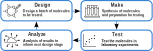
\includegraphics[width=\textwidth]{figures/dmta_cycle_v2.pdf}
      \caption{The Design-Make-Test-Analyze cycle is a key concept in drug discovery. The cycle
            consists of four stages: Design, Make, Test, and Analyze. Generative models can be used
            to design promising molecules to be tested. Computer-aided synthesis planning tools can
            be employed to make sure the molecules can be synthesized in the Make stage. The
            In the Analyze stage the experimental results can be used to update the property prediction
            models underlying the Design stage.
            \label{fig:dmta-cycle}}
\end{figure}
The hit discovery, hit-to-lead and lead optimization stages (blue box in
\Cref{fig:drug-discovery-pipeline}) usually operate in an iterative manner, resulting in a cycle of
choosing molecules to be tested, synthesizing them, testing them in laboratory experiments and
analyzing the results to guide the selection of the next molecule to be tested. This cycle is
usually referred to as the \ac{DMTA}-cycle:
\begin{itemize}
      \item \textbf{Design:} Under consideration of previous experimental results, the molecules to
            be tested are designed. The design generally aims to optimize the desired properties of
            the molecule, but also aims to maximize the information gained from the experiment.
      \item \textbf{Make:} The designed molecules are then synthesized and prepared for testing in
            the laboratory. This step requires a synthesis plan that outlines the steps needed to
            synthesize the molecule.
      \item \textbf{Test:} The synthesized molecules are then tested in laboratory experiments to
            measure the properties of interest. This can range from the activity of the molecule
            against a target, to its pharmacokinetic properties, to its toxicity and others.
      \item \textbf{Analyze:} The results of the experiments are analyzed. The obtained insights
            can then be used to guide the design of the next molecules to be tested.
            evaluation of the performance of the prediction models used in the design phase. The
            results of the analysis are then used to guide the design of the next molecule to be
            tested.
\end{itemize}

% TODO: Make this about ML
\subsection{Machine learning in drug discovery}
Computer-aided drug design (CADD) has long been an integral part of the pharmaceutical research and
development process. It encompasses a range of computational methods aimed at supporting and
enhancing drug discovery. While traditional CADD approaches have proven valuable, the integration of
machine learning (ML) has significantly expanded their capabilities.

Machine learning has become an important tool in modern CADD, offering new approaches for predicting
molecular properties and activities. ML models, trained on datasets molecular structures and their
associated properties, can screen chemical libraries to identify potential drug candidates, reducing
the time and resources required for experimental testing

Recent advances in deep learning have led to a surge in interested in generative models, introducing
new possibilities in drug discovery. These models expand the application of ML beyond property
prediction to the creation of novel molecular structures. Two key applications of generative models
in drug discovery are:

\begin{itemize}
      \item \textbf{De Novo Drug Design:} Generative models can create new molecular structures with specified property
            profiles, potentially expanding the chemical space explored in drug discovery. This approach allows
            for the generation of diverse compounds that may complement traditional design methods.
      \item \textbf{Computer-Aided Synthesis Planning:} Generative models are being applied to propose synthetic routes
            for target molecules, addressing a challenge in drug development. By suggesting potential synthesis
            pathways, these models aim to support the transition from in silico design to experimental
            realization.
\end{itemize}

The integration of generative models into the drug discovery pipeline represents a new approach,
offering additional tools for molecular design and synthesis planning. As these technologies
continue to develop, they may contribute to enhancing various aspects of the drug discovery process.

\section{Generative models in drug discovery}
\subsection{Molecular representations}
\begin{figure}
      \centering
      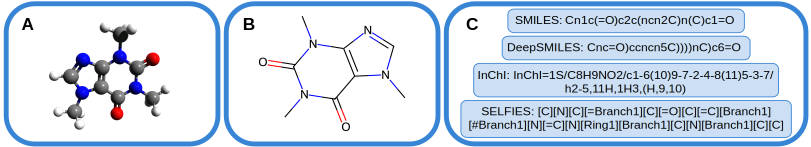
\includegraphics[width=\textwidth]{figures/representations/representations.pdf}
      \caption{Different ways to represent a caffeine molecule \textbf{A:}  The 3D structure of a
            molecule is given by the positions of its atoms in space. This structure is not
            necessarily fixed as some bonds can rotate and bonds can vibrate (Image source:
            \citep{EnglishCaffeine3D2010}). \textbf{B:} The graph representation of the same
            molecule. \textbf{C:} Smiles, DeepSmiles, SELFIES and InChI are line notations that
            linearize the molecules graph representation.\label{fig:molecular-graph}}
\end{figure}
Molecules, though fundamentally complex quantum mechanical entities, can be represented through
various simplified models for practical purposes. The most common representation depicts molecules
as graphs, where atoms are nodes and chemical bonds are edges. Figure \ref{fig:molecular-graph}b
shows a graph representation of caffeine. This graph structure captures the molecule's connectivity,
which defines its "identity". Additional properties such as atom type or charge are
incorporated as features of the nodes and edges. While this representation doesn't capture the full
quantum complexity, it provides a stable and practical framework for understanding and working with
molecular structures in many scientific and computational contexts.

Molecular graphs can be linearized into one-dimensional character sequences, known as line
notations. Figure \ref{fig:molecular-graph}c shows examples of various line notations. SMILES
(Simplified Molecular Input Line Entry System) \citep{weiningerSMILESChemicalLanguage1988} is a
widely used line notation that represents molecules as strings of characters. SMILES strings encode
the molecular graph in a human-readable format, making them convenient for storage and processing.
SMILES strings have proven particularly valuable for generative models, as they are easily processed
by sequence-based models like recurrent neural networks (RNNs) and Transformers
\citep{vaswaniAttentionAllYou2017}. Several extensions to SMILES have been proposed to make them
more amenable for use in machine learning models. DeepSmiles
\citep{oboyleDeepSMILESAdaptationSMILES2018} attempted to make it easier to generate syntactically
valid molecules, by changing the notation of branches and ring closures. SELFIES
\citep{krennSELFIESFutureMolecular2022} provide a representation of molecules in which any sequence
of tokens parses into a valid molecule. SAFE \citep{noutahiGottaBeSAFE2023} provides a
representation of molecules in which the substructures are represented by contiguous regions of a
SMILES string. InChI \citep{hellerInChIIUPACInternational2015} is less human-readable and less used
in machine learning contexts, but provides a non-proprietory representation of molecules, with
strict uniqueness and canonicalization rules.

Molecules can be represented in various complex forms beyond simple graphs and strings.
Three-dimensional structures provide a spatial description of a molecule, detailing atomic positions
in 3D space along with information about atom types and bonds. The most comprehensive representation
is the quantum mechanical wavefunction, which captures the full complexity of molecular behavior.
While these more sophisticated representations are valuable for modeling a wide range of molecular
properties and interactions, but are not covered in the rest of this thesis.

\subsection{Generation strategies}
There are several approaches to constructing up molecular graphs. These mainly depend
on the type of model used and the representation of the molecule.
Some of the most common approaches are shown in Figure~\ref{fig:generation-strategies} and
described below.

\textbf{Sequence-based autoregressive models} constitute one of the most popular approaches for
generating molecules. This approach makes use of a linearized representation of the molecule, such
as a SMILES string. Then the model generates the molecule by sampling one token at a time,
conditioned on the previously sampled tokens, similarly to how a language model generates text.
% The likelihood of sampling a sequence $x$ is thus modelled by $p(x; \theta) = \prod_{i=0}^n p(x_i |
%       x_{1:i-1}; \theta)$. The  $\theta$ can then be tuned to optimize the objectives
% described in the following sections.
Early work by \citep{seglerGeneratingFocusedMolecule2018} and
\citep{gomez-bombarelliAutomaticChemicalDesign2018} relied on recurrent neural networks (RNNs) to
generate SMILES strings. This approach has since been popular and there has been work on
string-based representations more suitable to generation
\citep{oboyleDeepSMILESAdaptationSMILES2018,krennSelfReferencingEmbeddedStrings2020,noutahiGottaBeSAFE2023},
parsing the molecules into specialized data structures
\citep{kusnerGrammarVariationalAutoencoder2017,jinJunctionTreeVariational2018} and using other deep
learning architectures such as transformers
\citep{vaswaniAttentionAllYou2017,noutahiGottaBeSAFE2023,schwallerMolecularTransformerModel2019,bagalMolGPTMolecularGeneration2022,mazuzMoleculeGenerationUsing2023}.

\textbf{Graph-based autoregressive models} work similarly to its sequence-based counterpart, but
instead of relying on a linearization of the molecule, they work directly on the graph representation
of the molecule. The model generates the molecular graph by iteratively adding nodes and edges to the
graph. The model can be trained in a similar manner to the string-based models, by
predicting the next node or edge given the current state of the graph. However, the specification of
possible actions is more complex than in the 1D case as there is no natural ordering of the
nodes and edges in the graph \citep{liuConstrainedGraphVariational2018,liLearningDeepGenerative2018,youGraphConvolutionalPolicy2019,cohen-karlikOvercomingOrderAutoregressive2024}.

\textbf{One-shot methods} are a class of models that generate molecules in one step, without the
need for an iterative generation process. These models generate an adjacency matrix and node feature
vector of a molecule in a single step. This is usually done by first generating a continous version
of the molecule and then discretizing it to a valid molecule \citep{decaoMolGANImplicitGenerative2018,madhawaGraphNVPInvertibleFlow2019}.

% https://www.frontiersin.org/journals/hematology/articles/10.3389/frhem.2024.1305741/full#h4
\textbf{Rule-based models} generate molecules by applying a set of pre-defined graph transformation rules to
combine molecular fragments. The BRICS \citep{degenArtCompilingUsing2008} method provides a set of
molecular fragments and rules how to meaningfully combine them. This enables the generation of new
molecules by combining these fragments. DOGS \citep{hartenfellerDOGSReactionDrivenNovo2012}
generates molecules by applying a set of chemical reaction rules to a set of starting molecules,
which has the advantage of biasing generation towards synthesizable molecules.\@
\citet{jensenGraphbasedGeneticAlgorithm2019} defines graph mutation and crossover operations to
generate new molecules. These models allow the generation of molecules that are chemically valid, or
resemble known ``reasonable'' molecules.


\subsection{Distribution-learning}
\begin{figure}
      \centering
      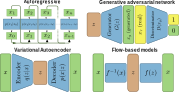
\includegraphics[width=0.9\textwidth]{figures/distribution-learning-models.pdf}
      \caption{Different types of distribution-learning models. All model types
            try to fit the data distribution $p(x)$, but differ in the way they achieve this goal.
            While autoregressive models and generative flows the exact likelihood of the data can be calculated,
            and optimized, VAEs rely on a variational approximation of the likelihood, and generative adversarial networks
            indirectly fit the data distribution using a game-theoretic approach. \label{fig:distribution-learning-models}}
\end{figure}
% Whats distribution learning
Distribution-learning is a fundamental application of generative models in drug design. Its
objective is to create a model that accurately captures the distribution of molecules within a
dataset. Formally, the model learns a distribution $q(x)$ that approximates the true distribution
$p(x)$ of molecules in a dataset. This approach enables the model to grasp both the syntax and semantics of the
molecules in the data. These models can be trained on large chemical libraries of stable
molecules, PubChem \citep{kimPubChemSubstanceCompound2016}, ChEMBL \citep{bentoChEMBLBioactivityDatabase2014} or
%TODO: Add zinc on mac https://pubs.acs.org/doi/full/10.1021/ci3001277
\citep{zinc}. Using this process the resulting models can learn what reasonable molecules look like
in the context of drug discovery. This makes them useful for their two main purposes: they can
expand virtual libraries and, more crucially, act as a foundation for other applications such as
goal-directed generation, which we will explore in the subsequent section.

% \begin{align} \mathcal{L} = - \mathbb{E}_{x \sim p(x)} \log q(x). \end{align}
In recent years there has been a surge in interest distribution-learning models based on deep neural
networks. Many architectures and training strategies originally proposed for text and image
generation have been adapted and specialized to generate molecules. While all of them aim to
approximate $p(x)$, they differ in the way they model the distribution and the choice of molecular
representation.

\paragraph{Autoregressive models} can be directly trained using a maximum likelihood approach by
minimizing the cross entropy or \ac{NLL} of the training data
\begin{align}
      \mathcal{L} = - \mathbb{E}_{x \sim p(x)} \log q(x) \approx - \frac{1}{N} \sum_{i=1}^N \log q(x_i),
\end{align}
where $q(x)$ is the model distribution and $p(x)$ is the true distribution of the data. These models
are explicit density models, as the likelihood for a given molecule can be calculated exactly.
Autoregressive models form the backbone of many generative models in drug discovery
\citep{gomez-bombarelliAutomaticChemicalDesign2018,seglerGeneratingFocusedMolecule2018,olivecronaMolecularDenovoDesign2017,guoAugmentedMemoryCapitalizing2023,thomasAugmentedHillClimbIncreases2022,jaquesSequenceTutorConservative2016,cohen-karlikOvercomingOrderAutoregressive2024,}

\paragraph{Variational autoencoders} (VAEs) \citep{kingmaAutoEncodingVariationalBayes2013} generate molecules by first
sampling from a simple latent distribution $p(z)$, and then mapping the samples to molecular space
via a probabilistic decoder network $p(x|z)$. To make training tractable a second network, the
encoder network $q(z|x)$ is used to map the data to the latent space. The model is then trained to
maximize the evidence lower bound (ELBO) of the data
\begin{align}
      \log p(x) \geq \mathbb{E}_{q(z|x)}[\log p(x|z)] - \text{KL}(q(z|x) || p(z)),
\end{align}
where KL is the Kullback-Leibler divergence. This model has the advantage of providing a continuous
latent space, which can be used to interpolate between molecules and allows the use continuous
optimization algorithms in latent space. VAEs belong in the class of approximate density models, as
the likelihood of a given molecule can be calculated approximately via monte carlo sampling. VAEs
have been a popular choice for generating molecules
\citep{gomez-bombarelliAutomaticChemicalDesign2018,kusnerGrammarVariationalAutoencoder2017,simonovskyGraphVAEGenerationSmall2018,samantaNeVAEDeepGenerative2018,jinJunctionTreeVariational2018,daiSyntaxDirectedVariationalAutoencoder2018,liuConstrainedGraphVariational2018}.


% moflow, graphnvp (has nice discussion on one-shot generation)
\paragraph{Generative flows} \citep{rezendeVariationalInferenceNormalizing2016} are based on the idea of learning a bijective mapping between molecular
space and a latent space. Generative flows transform from a simple distribution $p(z)$ in latent space
to a distribution in chemical space, p(x), via a bijective mapping $f: z \rightarrow x$.
The likelihood of the training data can then be directly calculated and optimized
via the change of variables formula:
\begin{align}
      p_x(x) = p_z(f^{-1}(x)) \left|
      \det \left[
      \left. \frac{\partial f^{-1}(v)}{\partial v} \right|_{v=x}
      \right]
      \right|.
\end{align}
Originally generative flows have been proposed for continuous data, but have been adapted to
discrete data such as molecules by using a continuous relaxation of the molecule
\citep{madhawaGraphNVPInvertibleFlow2019}. These models also belong to the class of explicit density
models, as the likelihood of a given molecule can be calculated exactly.

% molgan
\textbf{Generative adversarial networks} (GANs) \citep{goodfellowGenerativeAdversarialNetworks2014}
are latent space models that map a simple distribution in latent space to molecular space, but rely
on a game-theoretic approach to training. A generator network is trained to generate data, which is
then fed to a discriminator network. The two networks then engage in a minimax game, where the
discriminator is trained to distinguish between real and generated data, while the generator
is trained to generate samples that fool the discriminator.\@ \acp{GAN} are implicit density methods they sample from the
model distribution, but do not provide a likelihood for a given sample. This approach has been
combined with different generation strategies in the context of drug discovery \citep{decaoMolGANImplicitGenerative2018,kadurinDruGANAdvancedGenerative2017,guimaraesObjectiveReinforcedGenerativeAdversarial2017,mendez-lucioNovoGenerationHitlike2018,tangMolecularGenerativeAdversarial2024}

% \begin{figure}
%       \centering
%       \includegraphics[width=\textwidth]{./figures/goal_directed_cycle_and_virtual_screening.pdf}
%       \caption{Comparison of goal-directed generative models and virtual screening. Goal-directed
%             generation proceeds in a loop where already scored molecules inform what molecules to
%             test next. Virtual screening proceeds in a linear fashion, where the molecules to be
%             tested are determined beforehand. }
% \end{figure}


\subsection{Goal-directed molecule generation}
\begin{figure}
      \centering
      \includegraphics[width=0.8\textwidth]{./figures/goal_directed_generation_vs.pdf}
      \caption{Illustration of the difference between goal-directed molecule generation and virtual
            screening in a 2D chemical space, where each point represents a molecule. The
            background color represents the molecules' scores. Goal-directed generation works
            akin to a numerical optimization algorithm and efficiently finds high-scoring molecules,
            shown in the transition from red to blue stars. In contrast VS amounts to a random search in chemical space, which is less efficient
            and is likely to miss high-scoring regions of chemical space. \label{fig:goal-directed-generation}}
\end{figure}

% TODO: Add figure with different goal directed strategies
Goal-directed molecule generation \citep{schneiderNovoMolecularDesign2013} is a computational
approach for automatically designing molecules with desired property profiles. Goal-directed
generation expands upon \ac{VS}, a method in which a library of molecules is ranked according to the
output of a \ac{QSPR} model.\ \citet{waltersVirtualChemicalLibraries2019} estimates that
approximately $10^{13}$ molecules can be routinely tested in a \ac{VS} experiment. While this number
can vary significantly depending on the computational cost of running the \ac{QSPR} model, it is
dwarfed by the size of drug-like chemical space, which is estimated to contain between $10^{30}$ and
$10^{60}$ molecules \citep{waltersVirtualChemicalLibraries2019,ruddigkeitEnumeration166Billion2012}.
Consequently, \ac{VS} is limited to exploring only a small fraction of chemical space and cannot
fully leverage the vast number of possible candidates that drug-like chemical space offers.

% How does DNDD help
Goal-directed generators address this limitation of \ac{VS} by focusing the search on the most
relevant parts of chemical space. In contrast to the random search approach taken by \ac{VS},
goal-directed generators act more like optimizers that are able to efficiently locate maxima. This
is achieved by an iterative process in which a model generates a set of molecules, which are then
scored by a \ac{QSPR} model. These scores are then used to update the model, shifting the sampling
distribution to regions of chemical space with higher scores.

Recently, there has been a surge of deep learning-based goal-directed generators
\citep{eltonDeepLearningMolecular2019,sanchez-lengelingInverseMolecularDesign2018,duMachineLearningaidedGenerative2024}.
A multitude of different models have been proposed, which are based on a variety of neural network
architectures, training strategies and molecular representations. These methods augment traditional
rule-based generation approaches that have been combined with graph search and evolutionary
algorithms. \citep{schneiderComputerbasedNovoDesign2005,schneiderNovoMolecularDesign2013}. The new
wave of deep-learning methods has shown great promise in generating novel molecules with desired
property profiles and has led to success in a variety of applications, such as the design of new drugs,
materials or catalysts \citep{todo}.

Some of the most commonly used approaches to goal-directed molecular generation are:
\begin{itemize}
      \item \textbf{Hill-climbing}
            \citep{seglerGeneratingFocusedMolecule2018,xieMARSMarkovMolecular2021,thomasAugmentedHillClimbIncreases2022}
            is a simple optimization algorithm that relies on an underlying distribution-learning model.
            Molecules are sampled from the model's learned distribution and their scores are evaluated.
            The model is then retrained on the top-scoring molecules and the process is repeated.
      \item \textbf{Reinforcement learning} uses the molecule scores as a reward signal to update
            the model distribution. This is achieved through methods based on the REINFORCE algorithm
            \citep{williamsSimpleStatisticalGradientfollowing1992} which allows to update the model
            distribution in a way that increases expected scores of the generated molecules
            \citep{olivecronaMolecularDenovoDesign2017,thomasAugmentedHillClimbIncreases2022,youGraphConvolutionalPolicy2019,guoAugmentedMemoryCapitalizing2023}.
      \item \textbf{Genetic algorithms} in molecular generation operate by evolving an initial
            population of molecules through iterative cycles of mutation, crossover, and selection \citep{jensenGraphbasedGeneticAlgorithm2019,nigamGenerativeModelsSuperfast2021,yoshikawaPopulationbasedNovoMolecule2018}.
            Starting from an initial set of molecules, new molecules are generated by applying
            mutation and crossover operations. The molecules are then scored, and the best ones are
            selected for the next generation. This process is repeated for multiple generations,
            gradually optimizing the population towards desired molecular characteristics.
      \item \textbf{Tree search} methods build a tree of possible molecules by recursively applying a set of transformation rules
            to some initial molecules. Using techniques such as Monte Carlo Tree Search, the tree is
            explored to find the most promising molecules \citep{yangChemTSEfficientPython2017,jensenGraphbasedGeneticAlgorithm2019}.
      \item \textbf{Continuous optimization} employ classical optimization algorithms in the continuous
            latent space of (variational) autoencoders
            \citep{gomez-bombarelliAutomaticChemicalDesign2018,kusnerGrammarVariationalAutoencoder2017,winterEfficientMultiobjectiveMolecular2019}
            or generative flows \citep{madhawaGraphNVPInvertibleFlow2019}.
      \item \textbf{Generative Flow Networks} \citep{bengioFlowNetworkBased2021} aim to generate
            molecules with probability proportional to their score. This method relies on an
            iterative generation process and models chemical space as a directed acyclic graph, with
            nodes being intermediate molecules and edges graph edits. The transition probabilities
            between nodes are given by a "flow" of probability mass from the root node to finished
            molecules, such that the probability of each finished molecule is proportional to its
            score. This has the advantage of being able to explore multiple modes of the scoring
            function.
\end{itemize}

\subsection{Challenges in Evaluating Generative Models in de Novo Design}
\subsubsection{Evaluation of distribution-learning models}
The most basic and commonly used checks to assess the quality of the generated compounds are the
validity, uniqueness and novelty of the generated molecules. A molecule is valid if it obeys
chemical valence rules, which is usually checked using chemoinformatics toolkits such as RDKit
\citep{landrumRDKitOpensourceCheminformatics2006}. The uniqueness of a set of molecules measures the
fraction of unique molecules in the set and can flag models that output many duplicates. The novelty
a set of generated molecules is the fraction of molecules that are not in the training set and can,
to a certain extent, detect whether a model overfits to the training set.

A variety approaches exist to assess how well a model can learn the distribution of the training
set. Explicit/approximate density models allow principled evaluation using the negative
log-likelihood on a hold-out test set. However, this is not applicable for implicit density models
such as GANs. The KL-divergence between the distributions of scalar molecular properties (e.g.
molecular weight, logP, ...) of the generated molecules and the training set is a commonly used
metric to evaluate the distribution fit \citep{brownGuacaMolBenchmarkingModels2019}, but is usually
determined using a limited number of properties. The Frechet ChemNet Distance (FCD)
\citep{preuerFrechetChemNetDistance2018} provides a more comprehensive check of the distribution
fit. The FCD compares the distributions of the activations of a neural network trained to predict
bioactivities. The Frechet distance between the distributions of the activations of the generated
molecules has been shown to be sensitive to distributional differences in many different molecular
properties.

The MOSES \citep{polykovskiyMolecularSetsMOSES2020} and GuacaMol
\citep{brownGuacaMolBenchmarkingModels2019} benchmarks provide standardized frameworks for
evaluating distribution-learning models in molecular generation. While these benchmarks represent
progress in assessment methodology, questions remain about their comprehensiveness and ability to
fully capture the complexities of molecular generation tasks in drug discovery contexts.

\subsubsection{Goal-directed optimization of ML-based scoring functions}
Scoring functions based on machine learning models are commonly used in goal-directed generation
tasks \citep{todo}. The fact that such machine learning models are trained on limited amounts of
experimental data, adds additional aspects to a proper model evaluation. In this setting there
already are known molecules with high scores which are  used to train the scoring function. The task
thus becomes to find \emph{novel} high-scoring molecules using the ML model's generalization
capabilities. However, the machine learning models are often biased towards their training data,
which might lead to a lack of novelty in the generated molecules. It is not clear whether
this actually leads to a lack of novelty and how to quantify such biases.

Another issue is that optimizing an ML model's output with respect to its input can lead to
unexpected problems. Research has demonstrated that samples generated through this optimization
process can incorrectly receive high scores from the model, as shown in
\citep{szegedyIntriguingPropertiesNeural2014,goodfellowExplainingHarnessingAdversarial2015}. This
phenomenon occurs because discriminative models don't necessarily learn all characteristics of
high-scoring samples to perform classification. Instead, they often rely on a limited set of
correlations between the input sample and the target property.

Consequently, the model may classify
certain samples as high-scoring, even though they wouldn't actually score highly in reality. While
this effect was readily detectable in the image domain, where human vision can easily provide ground
truth evaluation, it's more challenging to identify in molecular optimization. It remains unclear
whether this issue extends to the context of goal-directed molecule generation and how to
quantitatively assess its impact in this field.

% The generated molecules may be outside the applicability domain of the scoring function, in which
% case the scores might become uninformative. In this case wet-lab validation is necessary to assess
% the quality of the generated molecules. While initially rare
% \citep{merkNovoDesignBioactive2018,merkTuningArtificialIntelligence2018} these early studies have
% since been complemented by more recent studies \citep{duMachineLearningaidedGenerative2024}.
% However, due to the cost of the training data, in-silico validation is still wide-spread in the
% literature.

\subsubsection{Diversity of generated molecules}
The diversity of the generated molecules is an important aspect in the application of goal-directed
generative models
\citep{martinDiverseViewpointsComputational2001,gorseDiversityMedicinalChemistry2006}. The used
scoring functions are usually only imperfect and incomplete approximations of the desired
properties. Given the expected failure of some of the candidates in later experiments, it is
important to generate diverse sets of molecules. Diversity encourages uncorrelated outcomes in
downstream experiments, which increases the chances of finding a successful candidate. In essence, a
varied molecular portfolio serves as a hedge against the inherent uncertainties in the modeling and
experimental processes.

% Bad diversity metrics
The concept of diversity in molecular generation is complex, with its measurement depending on the
specific problem at hand. While internal diversity (average pairwise distance between molecules) is
commonly used, it has proven inadequate for goal-directed generation
\citep{waldmanNovelAlgorithmsOptimization2000,xieMARSMarkovMolecular2021,thomasComparisonStructureLigandbased2021}.
\citet{thomasComparisonStructureLigandbased2021} proposed the sphere exclusion diversity (SEDiv)
metric, which aligns better with chemical intuition but can be misleading for differently sized
sets. \citet{xieHowMuchSpace2023} introduced the \#Circles metric, a non-normalized version of SEDiv,
which better addresses the needs in goal-directed generation. It does so by
by focusing on chemical space coverage of the generated molecules which correlates with
the probability of finding successful candidates.

While initial evaluations using \#Circles have been conducted, most comparisons are limited by the
fact that the models were not adapted to the diverse optimization setting. A comprehensive
comparison of models specifically designed for diverse optimization is still missing, leaving open
the question of how well different approaches perform in generating diverse, high-scoring molecules.

\subsubsection{Standardized Computational Resources}
A frequently neglected aspect in evaluating goal-directed models is the use of standardized
computational resources. At its core, optimizing molecular properties is a search problem
that—given unlimited resources—can be solved through exhaustive enumeration of the chemical space.
Consequently, the primary challenge in goal-directed generation lies in identifying high-scoring molecules
while minimizing resource consumption.

% Current literature
However, many studies compare different models without accounting for this crucial factor,
potentially leading to biased comparisons. For instance, some algorithms might run for days or
weeks, while others operate for mere minutes or hours. Recently, this issue has gained increased
attention, after \citep{gaoSampleEfficiencyMatters2022} proposed a benchmark that measures
the sample efficiency of goal-directed generation algorithms. Other researchers have adapted to this approach
\citep{thomasReevaluatingSampleEfficiency2022,thomasAugmentedHillClimbIncreases2022,guoAugmentedMemoryCapitalizing2023}.

% Whats missing 
Both of these aspects remain underexplored in the literature especially in the context of finding
diverse high-scoring molecules.

% Cross check with the paper
\subsection{Retrosynthesis prediction}
% Add figure of search tree 
Drug candidates, whether designed by generative models or other means, eventually need to be
synthesized for testing and eventually for use in patients. However, finding a synthesis route for a
given molecule can be a complex and time-consuming process. \Ac{CASP} methods help
chemists to find synthesis routes, enabling synthesis of previously inaccessible molecules or making
synthesis more efficient and cheaper.

This problem is often approached using a retrosynthesis approach
\citep{coreyComputerAssistedDesignComplex1969,coreyLogicChemicalSynthesis1991a}, which
recursively deconstructs the target molecule into simpler precursors until they match available
starting materials. At each step, single-step retrosynthesis prediction models suggest sets of
reactants that could theoretically combine to produce the current (intermediate) target molecule.
The success of retrosynthesis planning hinges on highly accurate chemical reaction models, as these
ensure that the proposed synthetic routes are feasible in laboratory conditions.

Early work in retrosynthesis prediction relied on carefully curated expert rules  encoding
possible reactions. Recently, machine learning models that learn the patterns of chemical reactions
from examples stored in reaction databases have received increased attention
\citep{coleyMachineLearningComputerAided2018}. One line of work relies on sequence-to-sequence
SMILES strings of reactants given that of the product, using models
originally developed for machine translation
\citep{schwallerMolecularTransformerModel2019,namLinkingNeuralMachine2016,schwallerFoundTranslationPredicting2018,karpovTransformerModelRetrosynthesis2019,tetkoStateoftheartAugmentedNLP2020}.
Another set of approaches exploit the fact that connectivity in a reaction is often preserved, and
use graph neural networks to edit the connectivity of the target molecule in order to yield possible
reactants \citep{sachaMoleculeEditGraph2020,shiGraphGraphsFramework2020,somnathLearningGraphModels2020,yanRetroXpertDecomposeRetrosynthesis2020}.

Template-based methods represent another approach to retrosynthesis prediction
\citep{seglerNeuralSymbolicMachineLearning2017,seglerPlanningChemicalSyntheses2018,daiRetrosynthesisPredictionConditional2020,sunEnergybasedViewRetrosynthesis2020}.
These models first extract a set of graph transformation rules, or templates, from a large reaction
database. These templates encode common reaction patterns. Given a target molecule ranks the
templates based on their likelihood of producing a feasible reaction. Finally, the highest-ranked
templates are applied to the target to yield sets of reactants.

While template-based methods have shown excellent performance in retrosynthesis prediction, they
face challenges with rare templates. Template extraction often leads to many templates being
represented by only a few training samples, resulting in a few-shot learning problem where models
struggle to perform well on these uncommon templates. While some strategies have been proposed
to alleviate this issue, such as data augmentation \citep{fortunatoDataAugmentationPretraining2020}
and specialized architectures and training objectives
\citep{daiRetrosynthesisPredictionConditional2020}, the problem remains a challenge in the field.

\section{Aims and Objectives\label{sec:aims-objectives}}
\subsection{Identifying Failure Modes in Generative Model Evaluation}
In \citep{renzFailureModesMolecule2019} we investigate possible failure modes in the evaluation of
distribution-learning and goal-directed generative models. We show that the distribution-learning
benchmark proposed in GuacaMol \citep{brownGuacaMolBenchmarkingModels2019} is not able to
distinguish recently published generative models from simple baseline models. We show that most of
the tested generative models do not outperform the simple baseline model, or only do so marginally.
While this does not necessarily mean that the generative models are not useful, it calls for a more
comprehensive evaluation of distribution-learning models, such as evaluations using the negative
log-likelihood of the test set when applicable.

% Todo rewrite this with phrasing above
In the context of goal-directed optimization we introduce \emph{control scores} that give
information whether the optimization leads to the generation of molecules that are biased towards the
training data and whether the optimization overfits to the used scoring function.
The control scores are obtained by retraining the scoring function on a hold-out set of the training
data or using a different random initialization.

We show that the generated molecules are biased towards the high-scoring molecules in the training
set, which might lead to a lack of novelty in the generated molecules. We also show that the
generative models are able to overfit to the scoring function's random initialization.
This might lead to an overestimation of the models' performance and might lead to the generation of
molecules that are not high-scoring in reality. The proposed control scores serve as a diagnostic
tool to detect these issues. \Cref{sec:failure-modes} reprints the corresponding publication.

\subsection{Diversity-based comparison of goal-directed generators\label{sec:divopt}} In
\citep{renzDiverseHitsNovo2024} we introduce a benchmark for diverse optimization
that addresses the above-mentioned issues. In this benchmark, we evaluate the diversity of the
generated molecules using a recently proposed diversity metric \#Circles
\citep{xieHowMuchSpace2023}. We compare the performance of diverse optimization approaches under two
different compute budgets, namely a fixed number of scoring function evaluations and a fixed time
budget. The first setting is relevant for applications where the cost of evaluating the scoring
function dominates the optimization process, while the second setting is relevant for scoring
functions that are cheap to evaluate. Using this setup we test 14 goal-directed optimization methods
and show how SMILES-based auto-regressive models dominate the benchmark. \Cref{sec:diverse-hits}
reprints the corresponding publication.

\subsection{Improving few-shot and zero-shot retrosynthesis prediction}
In \citep{seidlImprovingFewZeroShot2022} we propose a novel approach to template-based
retrosynthesis prediction. We use a multimodal learning approach that learns to associate relevant
templates to product molecules using a Modern Hopfield Network
\citep{ramsauerHopfieldNetworksAll2020}. Our model can leverage structural information about the
templates and can make use of similarities between them. This allows for improved generalization,
especially for templates with few training samples and even for unseen templates. This model is
several times faster than comparable methods and shows good predictive performance.
\Cref{sec:mhn-react} reprints the corresponding publication.

\section{List of publications\label{sec:publications}} This thesis comprises the work published in
the following papers:

\begin{itemize}
      \item \fullcite{renzFailureModesMolecule2019}
      \item \fullcite{renzDiverseHitsNovo2024}
      \item \fullcite{seidlImprovingFewZeroShot2022}
\end{itemize}

% give overview over my other publications
\paragraph{Other Publications} Besides the papers listed above, I have also contributed to the
following publications:

\begin{itemize}
      \item \fullcite{preuerFrechetChemNetDistance2018}
      \item \fullcite{renzUncertaintyEstimationMethods2019}
      \item \fullcite{hofmarcherLargescaleLigandbasedVirtual2020}
      \item \fullcite{renzLowCountTimeSeries2023}
\end{itemize}